%
% Complete documentation on the extended LaTeX markup used for Insight
% documentation is available in ``Documenting Insight'', which is part
% of the standard documentation for Insight.  It may be found online
% at:
%
%     http://www.itk.org/

\documentclass{InsightArticle}

\usepackage[dvips]{graphicx}
\usepackage{subfigure}

%%%%%%%%%%%%%%%%%%%%%%%%%%%%%%%%%%%%%%%%%%%%%%%%%%%%%%%%%%%%%%%%%%
%
%  hyperref should be the last package to be loaded.
%
%%%%%%%%%%%%%%%%%%%%%%%%%%%%%%%%%%%%%%%%%%%%%%%%%%%%%%%%%%%%%%%%%%
\usepackage[dvips,
bookmarks,
bookmarksopen,
backref,
colorlinks,linkcolor={blue},citecolor={blue},urlcolor={blue},
]{hyperref}


%  This is a template for Papers to the Insight Journal. 
%  It is comparable to a technical report format.

% The title should be descriptive enough for people to be able to find
% the relevant document. 
\title{Explicit Deformable Model in VTK}

% 
% NOTE: This is the last number of the "handle" URL that 
% The Insight Journal assigns to your paper as part of the
% submission process. Please replace the number "1338" with
% the actual handle number that you get assigned.
%
\newcommand{\IJhandlerIDnumber}{3251}

% Increment the release number whenever significant changes are made.
% The author and/or editor can define 'significant' however they like.
\release{0.00}

% At minimum, give your name and an email address.  You can include a
% snail-mail address if you like.
\author{J\'er\^ome Velut}
\authoraddress{jerome.velut@gmail.com}

\begin{document}

%
% Add hyperlink to the web location and license of the paper.
% The argument of this command is the handler identifier given
% by the Insight Journal to this paper.
% 
\IJhandlefooter{\IJhandlerIDnumber}


\ifpdf
\else
   %
   % Commands for including Graphics when using latex
   % 
   \DeclareGraphicsExtensions{.eps,.jpg,.gif,.tiff,.bmp,.png}
   \DeclareGraphicsRule{.jpg}{eps}{.jpg.bb}{`convert #1 eps:-}
   \DeclareGraphicsRule{.gif}{eps}{.gif.bb}{`convert #1 eps:-}
   \DeclareGraphicsRule{.tiff}{eps}{.tiff.bb}{`convert #1 eps:-}
   \DeclareGraphicsRule{.bmp}{eps}{.bmp.bb}{`convert #1 eps:-}
   \DeclareGraphicsRule{.png}{eps}{.png.bb}{`convert #1 eps:-}
\fi


\maketitle


\ifhtml
\chapter*{Front Matter\label{front}}
\fi


% The abstract should be a paragraph or two long, and describe the
% scope of the document.
\begin{abstract}
\noindent
This document describes a set of classes\footnote{It is a subset of the
vtkKinship library \url{http://github.com/jeromevelut/vtkKinship}} that 
designs a generic explicit deformable model in VTK. The iterative mechanism
is first introduced through an inheritance of the vtkPolyDataAlgorithm class. 
This vtkIterativePolyDataAlgorithm is then a based for an implementation of the
deformation. Two examples of deformation are presented through an inheritance of
this base class. The provided source code may be used to build a ParaView plugin
that harnesses the animation feature.
\end{abstract}

\IJhandlenote{\IJhandlerIDnumber}

\tableofcontents

The deformable models are part of a wide family of computer graphics methods.
They were initially proposed in the context of real physics simulation, 
in particular for solid and soft body deformations \cite{TER87,TER88.3}. One of the
applications concerns the segmentation task in image processing:
The snakes \cite{KAS87} are often cited as the seminal work that induced the
huge amount of existing paper today \cite{MON01}. The main idea was to minimize
an energy computed under a curve evolving in an image domain. A proposed 
implementation was a discretization of the steepest descent algorithm, which
led to an iterative displacement of each point related to a trade-off between
internal and external forces. The explicit deformable models refer to this 
iterative deformation of the geometry, as opposed to implicit deformable
models \cite{}.

In this paper, we focus on the iterative design of an explicit deformable 
model. First, we present the \verb!vtkIterativePolyDataAlgorithm! class, that 
inherits from \verb!vtkPolyDataAlgorithm!. It allows a VTK filter to iteratively
process the input until a number of iteration is reached. A step-by-step
mechanism is also implemented, bringing useful interactive capabilities
-especially inside ParaView-. Second, two specialisations are presented: a 
brownian movement and a deformable model, designed through two classes derived 
from \verb!vtkIterativePolyDataAlgorithm!. Finally, a ParaView plugin is 
provided and a short example is given in which the animation feature is used in 
order to interact with the deformable model.
%
\section{Making PolyData algorithms iterative}
%
\subsection{basics}
The design of the VTK library is based on a pipeline of data processing. The
modification of an input anywhere in the pipeline triggers the execution of the
whole remaining, downward processes. An obvious consequence is the 
impossibility to plug the output of a filter directly to an upward input 
'as is': this feedback connection will create in many cases an infinite loop.
However, it is possible to do almost everything in the execution method, as far
as the inputs are not modified. The first element of the deformable model suit
is a \verb!vtkPolyDataAlgorithm!-inherited class, namely 
\verb!vtkIterativePolyDataAlgorithm!. It implements a caching procedure and a 
special iteration mechanism.
%
\subsection{Caching the input}
%
In order to avoid a modification of the input, a call to 
\verb!vtkIterativePolyDataAlgorithm::RequestData! copy the first connection of 
the first input port into a CachedInput member under certain condition:
\begin{itemize}
 \item this is the first iteration (i.e. \verb!CurrentIteration! is false)
 \item the filter is asked to compute all the iteration at each Update (i.e.
   \verb!IterateFromZero! is true)
 \item Maximum number of iterations (variable \verb!NumberOfIterations!) has 
been set to zero
\end{itemize}
The copy is a performed by:
\begin{verbatim}
      // Copy input
      this->CachedInput->DeepCopy( inputMesh );
      // Reset current iteration
      this->CurrentIteration = 0;
      // User define initial condition
      this->Reset( inputVector ); 
\end{verbatim}
%
Here, \verb!inputMesh! points to the first input connection of the first port.
This copy implies that the \verb!CurrentIteration! is 0. Child classes should
overwrite the \verb!Reset! function in order to implement special initial 
states.
%
\subsection{Iterating}
%
While \verb!CurrentIteration! is less than \verb!NumberOfIterations!, the 
classical iterative process is performed :
\begin{itemize}
 \item transform the \verb!CachedInput! and name it \verb!IterativeOutput!
 \item Increment the \verb!CurrentIteration!
 \item copy the \verb!IterativeOutput! over \verb!CachedInput!
\end{itemize}
%
The manipulation of \verb!CachedInput! is implemented in the specialisations of 
\verb!vtkIterativePolyDataAlgorithm::IterativeRequestData!:
%
\begin{verbatim}
   while( this->CurrentIteration < this->NumberOfIterations )
   {
      // Effective call to the iterative algorithm. Child classes
      // should override this function
      this->IterativeRequestData( inputVector ); 

      this->CachedInput->DeepCopy( this->IterativeOutput );
      this->CurrentIteration ++;      
   }     
\end{verbatim}
%
Two important points are illustrated in these lines of code. First, it is the 
responsability of the \verb!IterativeRequestData! function to set the
\verb!IterativeOutput! data. Second, the algorithm will iterate from 
\verb!CurrentIteration! to \verb!NumberOfIterations!. It means that the whole
iterations are not necessarily computed, unless it is explicitely asked by 
setting \verb!IterateFromZero! to $1$. It is useful for a dynamic visualisation
of an iterative process.

The final step, in a VTK point of view, is to copy the iterative output over
the real output of the filter:
%
\begin{verbatim}
   vtkInformation *outMeshInfo = outputVector->GetInformationObject(0);
   vtkPolyData* outputMesh = vtkPolyData::SafeDownCast(
                             outMeshInfo->Get(vtkDataObject::DATA_OBJECT()));

   if( this->NumberOfIterations == 0 )
      outputMesh->DeepCopy( inputMesh );
   else
      outputMesh->DeepCopy( this->IterativeOutput );  
\end{verbatim}
%
In the case where \verb!IterateFromZero! is $1$, the iterative process could be 
resetted by setting \verb!NumberOfIterations! to 0:
\begin{itemize}
 \item the initial input cache is performed
 \item the output of the filter is set to inputMesh
\end{itemize}
%
\section{Explicit deformable model}
%
\subsection{Dynamic point warping}
%
A simple implementation of the deformation of a point set is realized in
\verb!vtkPolyDataIterativeWarp!. An internal pipeline made of brownian vectors
and point warping is built. The input of this pipeline is \verb!CachedInput!
and the \verb!IterativeOutput! is set to be the output of the warp filter.

A basic illustration may be found in \verb!Examples/IterativeWarp.cxx!. A point
cloud \verb!vtkPointSource! is passed through the 
\verb!vtkIterativePolyDataAlgorithm! and an infinite loop increments the 
number of iterations before rendering the output. The example may run for a 
while, as it doesn't iterate from zero at each update of the filter.
%
\subsection{Deformable mesh}
%
This iterative point warping is easily extended to an explicit deformable mesh
framework. Let the input be a polygonal mesh; let the warp vectors being 
computed from a second input volume: If the warp vectors point to a minimum of 
an energy, then each point of the mesh will convergence towards these minima.

The class \verb!vtkDeformableMesh! implements such a behaviour. The main 
difference between this one and \verb!vtkPolyDataIterativeWarp! is that the warp
vectors are not randomly generated. They are expected as a vector array inside 
a \verb!vtkImageData! given on input port 1.

Although the input mesh may include topological information, those are not taken
into account: Each point are moved independently from each other. It means that
it is not possible to introduce internal forces in the deformation process in 
this class. Another specialisation has to be implemented.

The example \verb!Examples/DeformableMesh.cxx! shows this deformable model 
evolving in a volume of size $64^3$, representing an ellipsoid of radius 
$(18,14,28)$ and centered in the volume. The external forces are computed in a 
classical fashion. Let $I$ be an intensity image, $\mathcal{S}$ the 3D Sobel
operator. The second input of the \verb!vtkDeformableMesh! is then 
$\mathcal{S}(|\mathcal{S}(I)|)$. The
input is an UV-sphere (\verb!vtkSphereSource!). Executing the example shows the
sphere deforming to an ellipsoid (figure~\ref{fig:deform-sphere}).
%
\begin{figure}
\centering
 \subfigure[$i=0$]{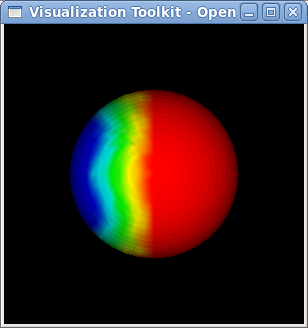
\includegraphics[width=0.3\textwidth]{./Figures/sphere-i0}}
 \subfigure[$i=100$]{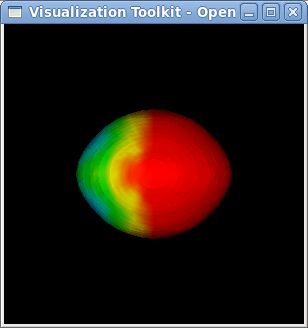
\includegraphics[width=0.3\textwidth]{./Figures/sphere-i100}}
 \subfigure[$i=250$]{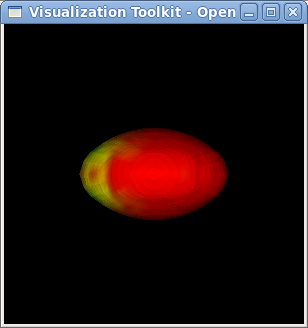
\includegraphics[width=0.3\textwidth]{./Figures/sphere-i250}}
\caption{Deformation of a spherical mesh towards an ellipsoid image at different
iterations $i$}
\label{fig:deform-sphere}
\end{figure}
%
\section{Paraview plugin}
%
The presented VTK classes are optionnally wrapped into a ParaView plugin. If 
the option ``BUILD\_PARAVIEW\_PLUGINS'' has been set to true during the CMake 
procedure, then the compilation will output a \verb!vtkPVExplicitDeformableModel!
dynamic library. This library is loadable in ParaView:
%
\begin{verbatim}
 "Tools" -> "Manage Plugins" -> "Load New ..."
\end{verbatim}
%
A new submenu \verb!Deformable model! appears in the \verb!Filters! menu, with
both \verb!Iterative Warp! and \verb!Deformable Mesh!.
%
\subsection{Basic pipeline}
%
The ParaView filters are directly linked to the VTK classes. The parameters have
then the same meaning. \verb!Deformable Mesh! is a multiple input filter: First,
the input mesh has to be selected and put as input of \verb!Deformable Mesh!.
Then, a dialog box will appear to ask for a second input containing Vectors.

When triggering the \verb!Apply! button, the iterative polydata filter will 
iterate internally until \verb!NumberOfIterations!.
%
\subsection{Rendering of successive iterations}
%
By harnessing the Animation View, it is possible to litteraly see the input mesh
or point cloud deforming, while keeping the usual interactions on the render 
window available. The screenshot in figure~\ref{fig:animation-view} shows the
settings of the animation view. The option \verb!IterateFromZero! is important
here, as it will avoid the computation of the whole iterations at each 
timestep.
%
\begin{figure}
 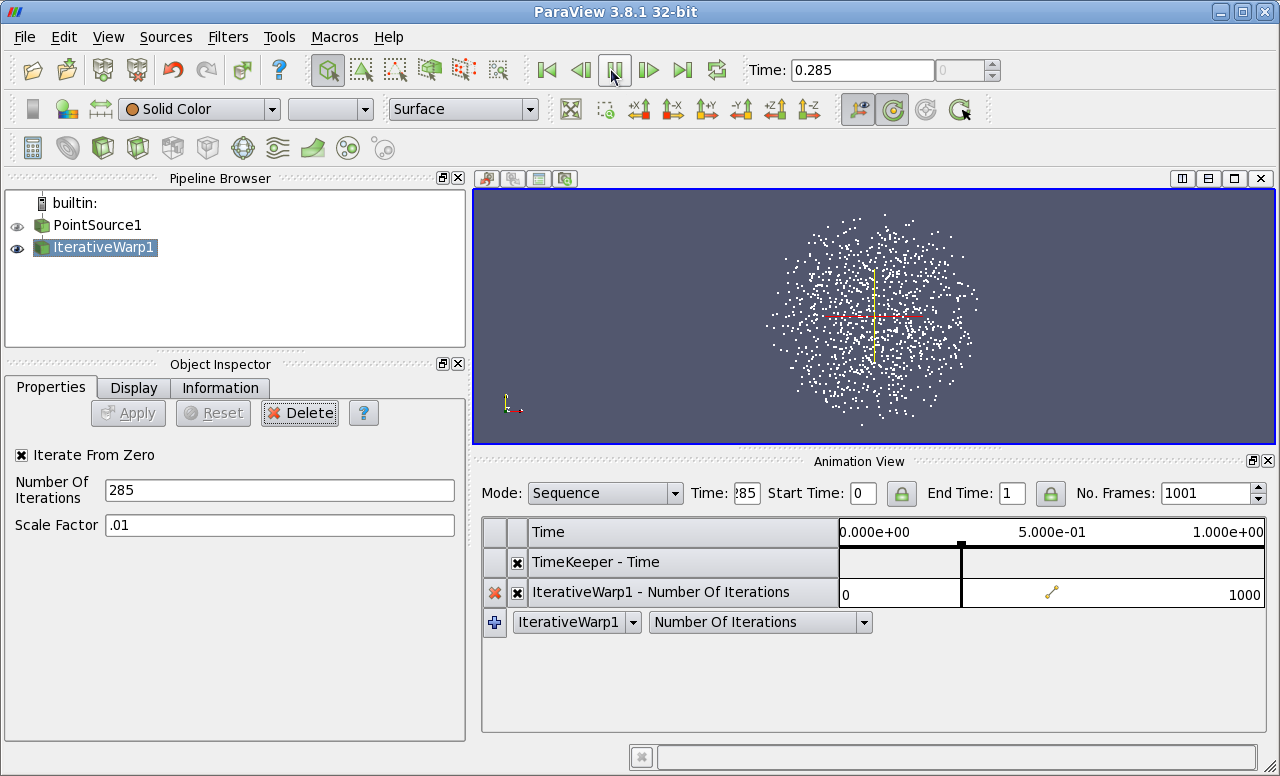
\includegraphics[width=\textwidth]{./Figures/animation-view}
\caption{Setting of the animation view to see the iterative deformation of the 
input PolyData}
\label{fig:animation-view}
\end{figure}
%
\section{Software Requirements}
%
This software has been successfully tested with ParaView-3.8.1 and ParaView-3.9
development branch on Linux Fedora 13.
%
\section{Conclusion}
%
We presented a set of classes that design the iterative deformation of a point
set. A generic class, inherited from \verb!vtkPolyDataAlgorithm! is derived to
specialise the deformation process. These deformable models are available in 
ParaView for interactive visualization of the deformation.

Future works will focus on the regularization of deformable meshes for a 
segmentation point of view, and the generalisation of input data structures.
%
\appendix

%%%%%%%%%%%%%%%%%%%%%%%%%%%%%%%%%%%%%%%%%
%
%  Insert the bibliography using BibTeX
%
%%%%%%%%%%%%%%%%%%%%%%%%%%%%%%%%%%%%%%%%%

\bibliographystyle{plain}
\bibliography{references}


\end{document}

